% This file was created by matplotlib2tikz v0.6.18.
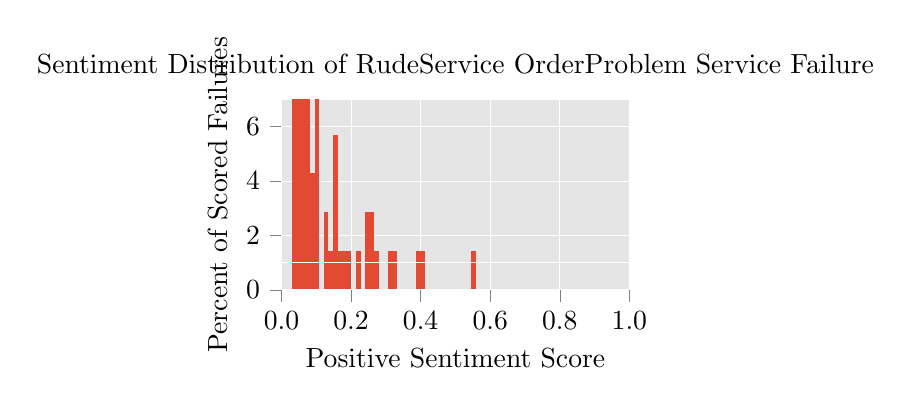
\begin{tikzpicture}

\definecolor{color0}{rgb}{0.886274509803922,0.290196078431373,0.2}

\begin{axis}[
axis background/.style={fill=white!89.80392156862746!black},
axis line style={white},
height=4cm,
tick align=outside,
tick pos=left,
title={Sentiment Distribution of RudeService
OrderProblem Service Failure},
width=6cm,
x grid style={white},
xlabel={Positive Sentiment Score},
xmajorgrids,
xmin=0, xmax=1,
xtick={0,0.2,0.4,0.6,0.8,1},
xticklabels={0.0,0.2,0.4,0.6,0.8,1.0},
y grid style={white},
ylabel={Percent of Scored Failures},
ymajorgrids,
ymin=0, ymax=7
]
\draw[fill=color0,draw opacity=0] (axis cs:0.0289683304727077,0) rectangle (axis cs:0.0421926006674767,7.13382549961907);
\draw[fill=color0,draw opacity=0] (axis cs:0.0421925932168961,0) rectangle (axis cs:0.055416863411665,7.13382449481614);
\draw[fill=color0,draw opacity=0] (axis cs:0.0554168671369553,0) rectangle (axis cs:0.0686411410570145,8.56058698225335);
\draw[fill=color0,draw opacity=0] (axis cs:0.0686411410570145,0) rectangle (axis cs:0.0818654075264931,9.9873571061912);
\draw[fill=color0,draw opacity=0] (axis cs:0.0818654000759125,0) rectangle (axis cs:0.0950896665453911,4.28029590265337);
\draw[fill=color0,draw opacity=0] (axis cs:0.0950896739959717,0) rectangle (axis cs:0.108313947916031,8.56058698225335);
\draw[fill=color0,draw opacity=0] (axis cs:0.108313947916031,0) rectangle (axis cs:0.121538214385509,0);
\draw[fill=color0,draw opacity=0] (axis cs:0.121538206934929,0) rectangle (axis cs:0.134762465953827,2.85353060176891);
\draw[fill=color0,draw opacity=0] (axis cs:0.134762480854988,0) rectangle (axis cs:0.147986754775047,1.42676449704223);
\draw[fill=color0,draw opacity=0] (axis cs:0.147986754775047,0) rectangle (axis cs:0.161211028695107,5.7070579881689);
\draw[fill=color0,draw opacity=0] (axis cs:0.161211043596268,0) rectangle (axis cs:0.174435302615166,1.4267661047276);
\draw[fill=color0,draw opacity=0] (axis cs:0.174435287714005,0) rectangle (axis cs:0.187659561634064,1.42676449704223);
\draw[fill=color0,draw opacity=0] (axis cs:0.187659561634064,0) rectangle (axis cs:0.200883835554123,1.42676449704223);
\draw[fill=color0,draw opacity=0] (axis cs:0.200883835554123,0) rectangle (axis cs:0.214108109474182,0);
\draw[fill=color0,draw opacity=0] (axis cs:0.214108109474182,0) rectangle (axis cs:0.22733236849308,1.4267661047276);
\draw[fill=color0,draw opacity=0] (axis cs:0.22733236849308,0) rectangle (axis cs:0.240556642413139,0);
\draw[fill=color0,draw opacity=0] (axis cs:0.240556657314301,0) rectangle (axis cs:0.253780901432037,2.85353220945519);
\draw[fill=color0,draw opacity=0] (axis cs:0.253780901432037,0) rectangle (axis cs:0.267005175352097,2.85352899408445);
\draw[fill=color0,draw opacity=0] (axis cs:0.267005205154419,0) rectangle (axis cs:0.280229479074478,1.42676449704223);
\draw[fill=color0,draw opacity=0] (axis cs:0.280229449272156,0) rectangle (axis cs:0.293453723192215,0);
\draw[fill=color0,draw opacity=0] (axis cs:0.293453752994537,0) rectangle (axis cs:0.306678026914597,0);
\draw[fill=color0,draw opacity=0] (axis cs:0.306677997112274,0) rectangle (axis cs:0.319902271032333,1.42676449704223);
\draw[fill=color0,draw opacity=0] (axis cs:0.319902271032333,0) rectangle (axis cs:0.33312651515007,1.42676771241659);
\draw[fill=color0,draw opacity=0] (axis cs:0.333126544952393,0) rectangle (axis cs:0.346350818872452,0);
\draw[fill=color0,draw opacity=0] (axis cs:0.346350789070129,0) rectangle (axis cs:0.359575062990189,0);
\draw[fill=color0,draw opacity=0] (axis cs:0.359575092792511,0) rectangle (axis cs:0.37279936671257,0);
\draw[fill=color0,draw opacity=0] (axis cs:0.372799336910248,0) rectangle (axis cs:0.386023610830307,0);
\draw[fill=color0,draw opacity=0] (axis cs:0.386023640632629,0) rectangle (axis cs:0.399247914552689,1.42676449704223);
\draw[fill=color0,draw opacity=0] (axis cs:0.399247884750366,0) rectangle (axis cs:0.412472158670425,1.42676449704223);
\draw[fill=color0,draw opacity=0] (axis cs:0.412472158670425,0) rectangle (axis cs:0.425696402788162,0);
\draw[fill=color0,draw opacity=0] (axis cs:0.425696432590485,0) rectangle (axis cs:0.438920706510544,0);
\draw[fill=color0,draw opacity=0] (axis cs:0.438920676708221,0) rectangle (axis cs:0.452144950628281,0);
\draw[fill=color0,draw opacity=0] (axis cs:0.452144980430603,0) rectangle (axis cs:0.465369254350662,0);
\draw[fill=color0,draw opacity=0] (axis cs:0.46536922454834,0) rectangle (axis cs:0.478593498468399,0);
\draw[fill=color0,draw opacity=0] (axis cs:0.478593528270721,0) rectangle (axis cs:0.491817802190781,0);
\draw[fill=color0,draw opacity=0] (axis cs:0.491817772388458,0) rectangle (axis cs:0.505042016506195,0);
\draw[fill=color0,draw opacity=0] (axis cs:0.50504195690155,0) rectangle (axis cs:0.518266260623932,0);
\draw[fill=color0,draw opacity=0] (axis cs:0.518266320228577,0) rectangle (axis cs:0.531490564346313,0);
\draw[fill=color0,draw opacity=0] (axis cs:0.531490564346313,0) rectangle (axis cs:0.544714868068695,0);
\draw[fill=color0,draw opacity=0] (axis cs:0.544714868068695,0) rectangle (axis cs:0.557939112186432,1.42676771241659);
\path [draw=white, fill opacity=0] (axis cs:0,0)
--(axis cs:0,7);

\path [draw=white, fill opacity=0] (axis cs:1,0)
--(axis cs:1,7);

\path [draw=white, fill opacity=0] (axis cs:0,0)
--(axis cs:1,0);

\path [draw=white, fill opacity=0] (axis cs:0,1)
--(axis cs:1,1);

\end{axis}

\end{tikzpicture}